\chapter{The Physics of OCE}\label{oce}

Elastography in general uses an underlying imaging modality to capture images of a sample undergoing mechanical loading, and estimates the sampel deformation (and hence sample mechanical properties) from these images. In particular, \ac{oce} utilises \ac{oct} as the underlying modality to producex high resolution images. \ac{oct} as an imaging technique is discussed in \autoref{oct}, followed by \ac{oce} as a connected application of \ac{oct} and elastography in \autoref{application_elastography}. 
This work focuses on the \ac{oce} technique in use at \ac{britelab}, which is based on phase-sensitive detection of compressive loading, and is discussed in detail in \autoref{compression_oce}.

\section{Optical Coherence Tomography}\label{oct}
\ac{oct} detects the light reflected from scatterers within a tissue, producing spatially localised intensity information by interference with a reference beam, enabling depth-resolved reconstruction of the location of the scatterers within the sample \cite{chin_parametric_2016}. Because the wavelength of light in tissue is significantly smaller than that of sound, \ac{oct} offers a much higher spatial resolution than ultrasound, on the order of $5-15 \mu m$ \cite{kennedy_emergence_2017}, as limited by the coherence length of the light source \cite{huang_optical_1991}. However, this higher resolution comes at the expense of depth of penetration into the tissue, which for \ac{oct}, is only 1-2mm beneath the surface \cite{schmitt_optical_1999}, in comparison to the relatively deep imaging capabilities of ultrasound.

\begin{figure}
	\centering
    \begin{subfigure}{0.47\textwidth}
    	\centering
        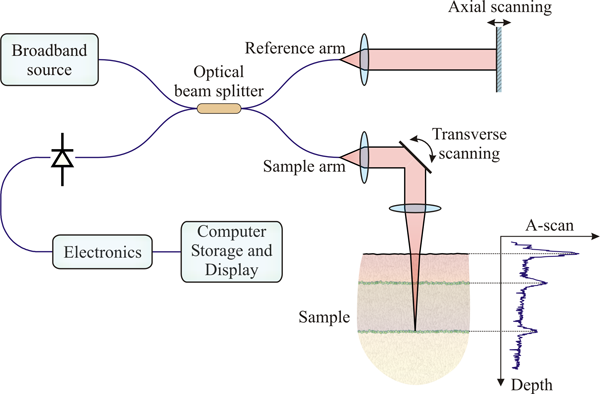
\includegraphics[width=\textwidth]{bground_figs/time_domain}
    \end{subfigure}
    \quad
    \begin{subfigure}{0.47\textwidth}
    	\centering
        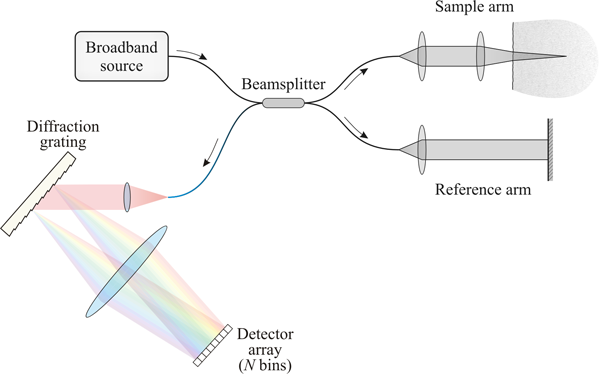
\includegraphics[width=\textwidth]{bground_figs/fourier_domain.png}
    \end{subfigure}
	\caption{Set ups for a) time-domain and b) Fourier-domain \ac{oct} systems. Taken from \cite{optical+biomedical_engineering_laboratory_introduction_nodate}.}
    \label{oct_domains}	
\end{figure}

%\subsection{Speckle in \ac{oct}}
\ac{oct} is a coherent imaging technique that relies on detecting constructive interference of a broadband light source, to produce an intensity field in depth. Constructive interference is only detected when the pathlength of the reflected field matches that of the reference to within the coherence length of the light source \cite{wijesinghe_improving_2017}, which defines the system spatial resolution. 

The interference pattern is dependent on the summation of multiple light fields, which interfere both constructively and destructively, therefore a characteristic mottled pattern appears in \ac{oct} images known as speckle \cite{wijesinghe_improving_2017}. Speckle produces highly variable \ac{oct} \ac{snr} by nature, therefore it is common to perform averaging on the measured signal to reduce variation. 

%\subsection{Time and Fourier-Domain \ac{oct}}
Time-domain \ac{oct} uses a simple low coherence Michelson interferometer set up, as seen in \autoref{oct_domains}, where the interference signal is measured between the light reflecting from the tissue, and an scanned reference mirror that changes the depth imaged \cite{huang_optical_1991}. The scanning of the reference mirror to image into the tissue produces a 1D A-scan, that contains information about the detected irradiance of the interferometer as a function of depth. Taking multiple A-scans across by moving laterally across a sample surface produces a 2D B-scan. Multiple B-scans can be used as cross-sections to build up an entire 3D scan volume, otherwise known as a C-scan. These descriptions are taken from those conventionally utilised in ultrasound imaging. The disadvantage of this set up are long acquisition times for the imaging of 3D volumes.

In contrast, Fourier-domain \ac{oct} systems remove the need for a scanning mirror, and allows imaging of an entire A-scan with one detection event based on principles of spectral interferometry \cite{chin_parametric_2016}. Rather than detecting the reflected intensity as a function of depth as in time-domain \ac{oct}, it is detected as a function of wavenumber of a broadband or swept frequency light source. The Wiener-Khinchin theorem dictates that the inverse Fourier transform of this measured spectral density provides the complex coherence function at different depths along the A-scan line \cite{schmitt_optical_1999}, from which the \ac{oct} signal is derived. The speed up using Fourier-domain \ac{oct} compared to time-domain \ac{oct} allows the imaging of 3D volumes, of approximately 10mm $\times$ 10mm $\times$ 2mm to be acquired in less than 1 second \cite{kennedy_emergence_2017}. The benefit of Fourier-domain \ac{oct} over time-domain is not only in allowing a much faster acquisition time, but also a more accurate detection of the complex signal. While it is possible to image phase information using time-domain \ac{oct} systems, mechanical jitter introduced by the reference mirror scanning makes this difficult \cite{wijesinghe_improving_2017}.

%\subsection{\ac{snr} in \ac{oct}}
Since the intensity pattern measured by the \ac{oct} signal is dependent on the intensity of the constructive interference with the reference and backscattered light field, a higher intensity implies a better match, and suggests that the estimate of displacement in that region more accurately points to the location of the scatterers within the volume. For regions of high \ac{oct} intensity, where the \ac{snr} $>>$ 1, the variance of the phase component of the complex signal is given by \cite{goodman_statistical_2015}:

\begin{equation}
	\sigma^2_{\Delta\phi_i} = \frac{1}{\text{SNR}}
	\label{snr_variance}
\end{equation}

\section{Application to Elastography}\label{application_elastography}

\ac{oce} is the combination of elastography with an \ac{oct} imaging system, as first proposed by Schmitt in 1998 \cite{schmitt_oct_1998}. The micro-architecture of tissue carries important information about disease states \cite{fung_biomechanics_1981}, however these are poorly demonstrated utilising only optical contrast. Using elastography with \ac{oct} as the underlying imaging modality allows high resolution mechanical contrast imaging on scales previously inaccessible to ultrasound and MRI-based elastography techniques. Of particular interest in this project is compressive \ac{oce} utilising phase-sensitive detection. Other techniques exist that may be utilised also to detect tissue displacement, such as speckle tracking via cross-correlation algorithms \cite{kennedy_review_2014}. However the advantage of phase-sensitive detection, which owes its origin to Doppler imaging in \ac{oct}, is in superior resolution and sensitivity (as set by the optical wavelength, therefore on the nanometre scale) compared to other techniques. 

\section{Phase-Sensitive Compression \ac{oce}}\label{compression_oce}    
\begin{figure}
	\centering
	\begin{subfigure}{0.4\textwidth}
    		\centering
        	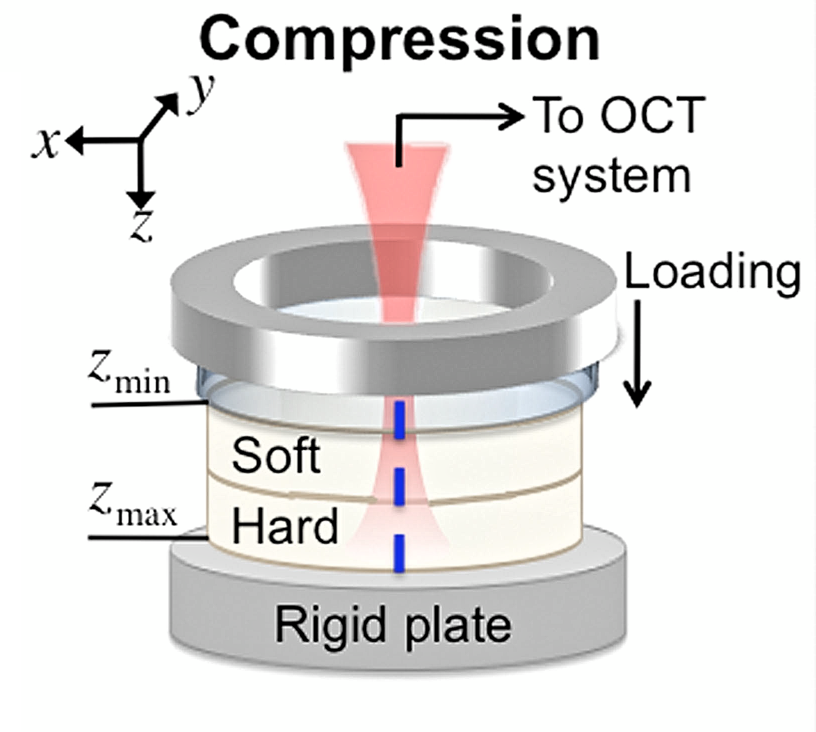
\includegraphics[width=\textwidth]{bground_figs/oce_hardware.png}
    	\end{subfigure}
   	\begin{subfigure}{0.3\textwidth}
    		\centering
	        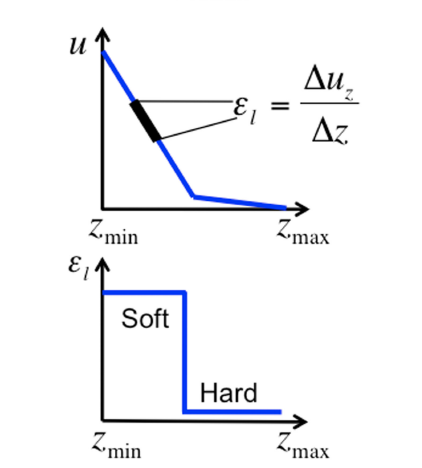
\includegraphics[width=\textwidth]{bground_figs/ascan_example.png}
	\end{subfigure}
	\caption{Compression OCE system, adapted from \cite{kennedy_review_2014}.}
	\label{oce_system}
\end{figure}

Compression \ac{oce} systems introduce a mechanical load to the sample by applying force to it in the axial direction, which results in displacement of the tissue, dependent on its constituent elastic properties. The typical system set up can be seen in \autoref{oce_system}. The tissue is first preloaded (compressed) to ensure good even contact with the loading mechanism (the sample window in \autoref{oce_system}). From here, a controlled step-load is applied using either an actuator or a translation stage. The \ac{oce} system show in \autoref{oce_system} is constructed in common-path mode, meaning the reflection at the interface of the sample with the imaging window is used as the reference reflector. 

Compression \ac{oce} produces a displacement field in the tissue, that can be measured in order to calculate the strain. The local strain is estimated as the spatial derivative of these displacements with respect to depth \cite{kennedy_review_2014} over a given axial fit window. 

Compressive loading techniques provide only qualitative comparison in strain elastograms, since it the resulting strain is dependent on the amount of compressive loading applied to the tissue. It is possible to produce quantitative elastogram images by measuring the stress locally applied to the sample by introducing a known stress layer above the imaged sample, as discussed in detail in \cite{kennedy_quantitative_2015}, however this will not be discussed further here. The benefit of compression techniques is their fast acquisition speeds for entire 3D volumes, as well as their ability to be extended to needle based \ac{oce} systems for imaging deep within the tissue \cite{kennedy_review_2014}. 

%\section{Phase-Sensitive Displacement Measurement}\label{phase_sensitive}
For phase-sensitive detection, the displacement induced by the step-loading is directly related to the phase difference between an unloaded and loaded scan, as in \autoref{phasedif_displacement} \cite{kennedy_strain_2012}. A limitation of phase-sensitive detection however is that only displacement co-axial to the imaging beam may be measured, which corresponds to axial strain only \cite{wijesinghe_improving_2017}. As mentioned, 

As mentioned in \autoref{compression_oce}, large variations in \ac{oct} \ac{snr} due to speckle produces spatially varying phase values, that are often averaged to improve the overall displacement sensitivity. This is commonly performed using a Kasai estimator \cite{zaitsev_hybrid_2016} \cite{wijesinghe_improving_2017} to perform weighted averaging on the complex number. The phase difference using this is then:

\begin{equation}
	\Delta\phi = \text{angle}\bigg( \frac{1}{n} \sum_\Omega A_i^{(k)} \cdot \text{conj}(A_i^{(l)}) \bigg)
	\label{kasai_estimate}
\end{equation}

Where $A$ is the complex number associated with the \ac{oct} image for the loaded ($k$) and unloaded ($l$) scans, $\Omega$ corresponds to the spatial window across which the phase is averaged, and $n$ the number of data points in that region.

\section{Strain Elastogram Image Formation}

The phase difference described in \autoref{kasai_estimate} above is calculated by buffering B-scan images in the data and averaging over a spatial region in the y-direction. Although the raw phase is random at each point in space, the change in phase is directly proportional to the displacement of the tissue at that location, as per \autoref{phasedif_displacement}:

\begin{equation}
	u_i = \frac{\lambda_0 \Delta\phi_i}{4\pi n}
	\label{phasedif_displacement}
\end{equation}

\subsection{Phase Unwrapping}

A significant limitation of phase-sensitive detection is that the measured phase can only take values in the interval $[0,2\pi]$. This results in wrapping of the phase difference as seen in \autoref{phase_wrapping} and if uncorrected, will result in discontinuities in the calculated displacement field.

To prevent phase wrapping in phase-sensitive displacement measurements, the difference in displacement between loaded and unloaded scans must be limited to approximately 0.3-0.46$\mu$m \cite{kennedy_optical_2014}. However in most instances, the amount of compression applied in \ac{oce} in order to produce images with sufficient contrast results in displacements large enough to induce phase wrapping in the signal. 

One approach to correcting for phase wrapping is to implement a phase unwrapping algorithm that loops through the data set and detects wrapping events. 

\begin{figure}[hb!]
	\centering
	\begin{subfigure}{0.49\textwidth}
		\centering
		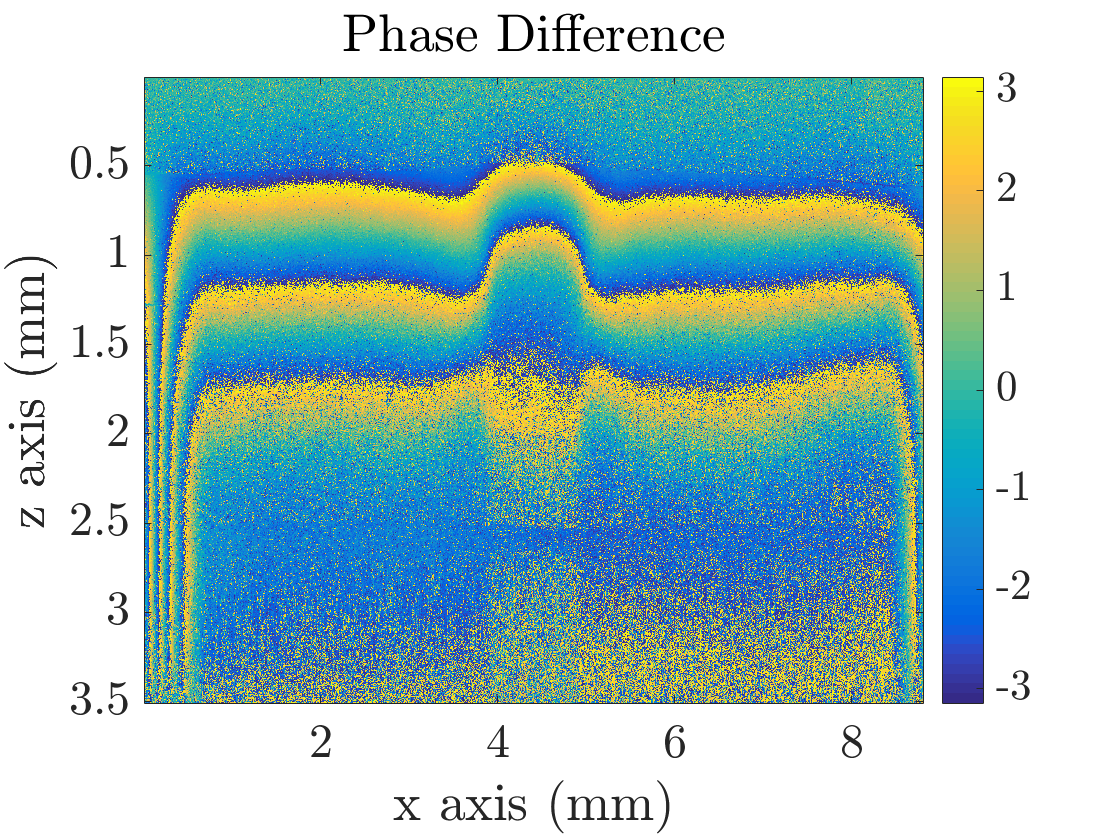
\includegraphics[width=\textwidth]{bground_figs/phase_difference.png}
	\end{subfigure}
	\begin{subfigure}{0.49\textwidth}
		\centering
		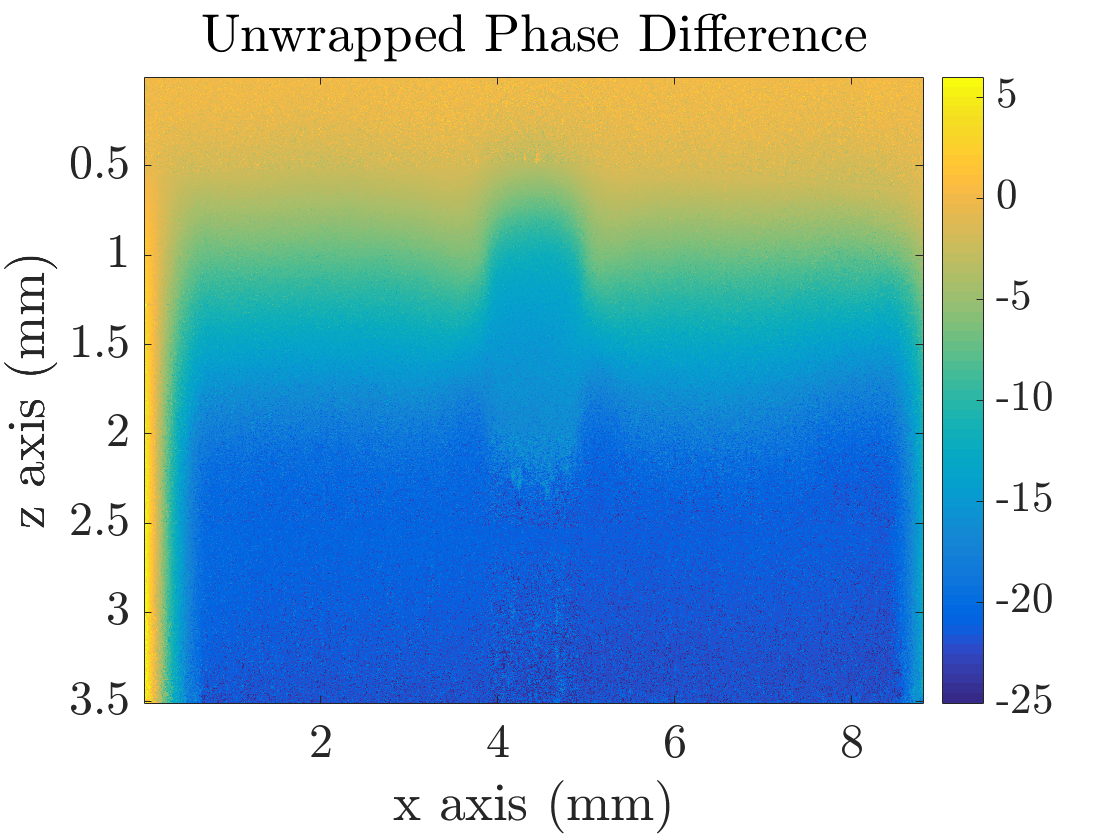
\includegraphics[width=\textwidth]{bground_figs/unwrapped_phase.png}
	\end{subfigure}
	\caption{Phase unwrapping demonstrated in a phantom scan data set in a) followed by the unwrapped phase difference b) computed using the unwrapping algorithm from \cite{kennedy_optical_2014}.}
	\label{phase_wrapping}	
\end{figure}

This algorithm is more completely described in the paper \cite{kennedy_optical_2014} (see section 2.5) however at a high level, it works under the assumption that displacements induced at a given depth is uniform over a local region, and performs first axial then lateral unwrapping. The phase difference is assumed to be unwrapped over an initial depth segment, for which a mean phase value is calculated. From here, each subsequent voxel in depth has an integer number of $2\pi$ subtracted from it based on minimising the difference between its phase value and the preceding mean value, in order to axially unwrap. The lateral unwrapping is performed in a similar way, except by minimizing the difference between the phase at a given voxel with the averaged phase of its lateral neighbours. It has been demonstrated that the algorithm can remove up to 5 wrapping discontinuities \cite{kennedy_optical_2014} before artefacts become prominent. The benefit of the phase unwrapping algorithm is that it is capable of returning the reconstructed displacement field of the entire B-scan. 

\subsection{Phase Offset Correction}

\begin{figure}[b!]
	\centering
	\begin{subfigure}{0.25\textwidth}
		\centering
		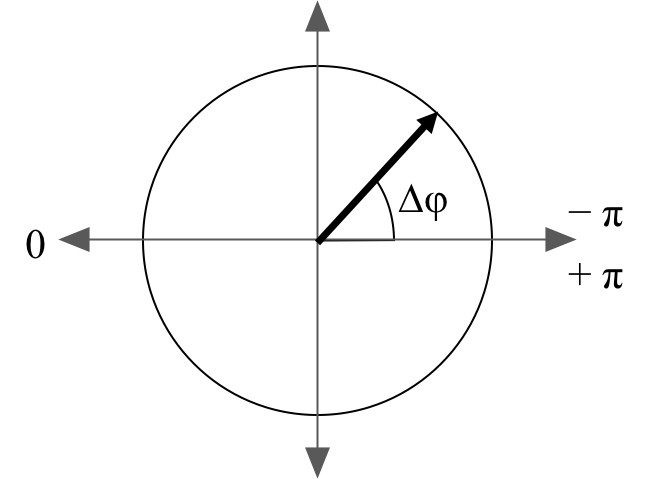
\includegraphics[width=\textwidth]{bground_figs/cplx_phasedif_phasor.png}
	\end{subfigure}
	\quad
	\begin{subfigure}{0.25\textwidth}
		\centering
		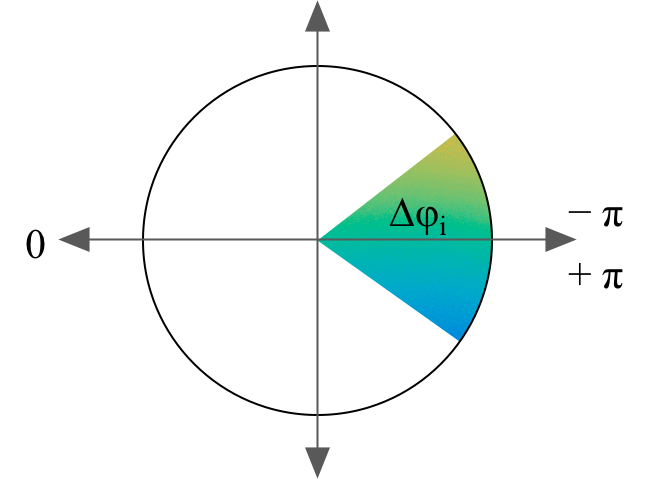
\includegraphics[width=\textwidth]{bground_figs/cplx_phasedif_segment.png}
	\end{subfigure}
	\quad
	\begin{subfigure}{0.25\textwidth}
		\centering
		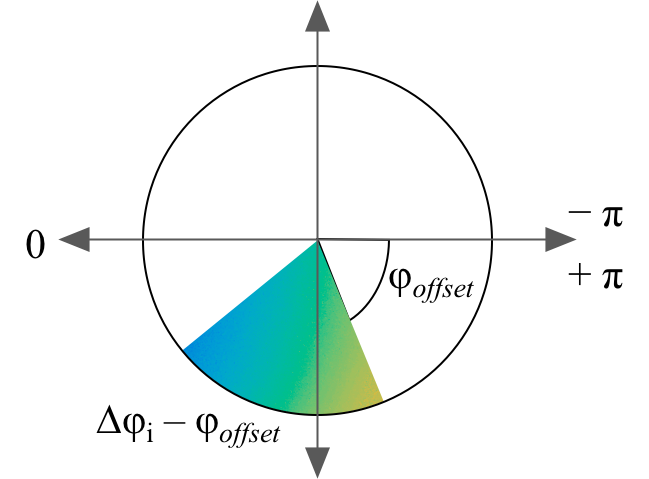
\includegraphics[width=\textwidth]{bground_figs/cplx_segment_shifted.png}
	\end{subfigure}
	\caption{The complex phase difference signal using phasor representation in a) as a single data point, b) as a fit window of phase difference data points wrapped around the $\pi/\pi$ discontinuity, and c) those data points shifted to an unwrapped region, based on application of a phase offset \cite{zaitsev_hybrid_2016}.}
	\label{phase_offset}	
\end{figure}

An alternative approach to the phase wrapping issue investigated by Zaitsev \textit{et al} \cite{zaitsev_hybrid_2016} is based around the fact that the underlying displacement field does not have to be extracted over the entire scan to produce a strain elastogram, but only the gradient within the fitting window must be maintained in order to produce a value for local strain. This allows the phase unwrapping algorithm to be dropped, and a complex phase offset is subtracted from each fit segment to remove any possible wrapping event by returning it to an unwrapped region, as shown in \autoref{phase_offset}. From here the strain is estimated using the unwrapped fit segment. This method obviously falters when there are multiple wrapping discontinuities within a given strain fit window. A further limitation is that subtraction of a complex phase offset is a non-linear filter operation, and therefore must be performed on each fit segment separately. This introduces processing bottlenecks.

%\subsection{Alternative Approaches}
A third range of approaches do not tackle the issue of phase unwrapping directly, but rather makes the fit segment so small it is assumed no wrapping can occur between. Using \ac{fd} of the complex phase with depth to calculate the strain ensures that no wrapping artefacts enter the image, provided that no wrapping events occur between consecutive pixels (which is unlikely given the load applied). 

\subsection{Strain Estimation}

From the processed phase difference data, the strain is estimated as the spatial derivative of the displacement in the axial direction. For phase wrapping approaches that utilise small fit windows as described in the previous section, noisy derivative estimates are produced that result in significant degradation of image quality when used alone. Other techniques that operate on unwrapped phase values (and hence a reconstructed displacement field) apply more detailed derivative estimations based on least squares regression approaches, aimed at minimising this noise.

These derivative estimators can be thought of as differentiation filters, or in this instance, strain filters \cite{lindop_general_2008} \cite{varghese_theoretical_1997}. The following chapter discusses a variety of strain filters from the literature in more detail.
